\section{Invariant Graph Embeddings}

We first motivate and argue in favor of particular form of ``fairness'' (or rather {\em invariance}) within the context of graph embeddings.
Following this, we outline our compositional and adversarial approach for enforcing these invariance constraints on graph embeddings. 

\subsection{Pragmatic fairness as invariance}

As noted in Section \ref{sec:relatedfair}, there are a multitude of definitions of algorithmic fairness in the literature---each definition with its own benefits and drawbacks.
Thus, rather than developing yet another new metric---or diving into thorny debates regarding the pros and cons of different formulations---in this work we instead consider a simple, user-centric formulation within the context of social graph embeddings.
Using gender as an example of a sensitive attribute and movie recommendation as an example relation prediction task, our approach is guided by the following question: {\em If one gives a user a button that says ``Please ignore my gender when recommending movies'', what does a user expect from the system after this button is pressed?}
Here, we accept it as non-controversial that the expectation from the user is that recommendation does not depend in any way on their gender, i.e., that the recommendation would be the same regardless of their gender.
Formally, given a user $u$, this expectation amounts to an assumption of independence, 
\begin{equation}\label{eq:edgeind}
  s(e) \perp a_u \qquad \forall v \in \V, r \in \R
\end{equation}
between the recommendation---i.e., the score of the edge, $s(e) = s(\langle \mb{z}_u, r, \mb{z}_v\rangle)$---and the sensitive attribute $a_u$.

One issue in directly enforcing Equation \eqref{eq:edgeind} is that there are many (potentially millions) of possible edges that we might want to score for every node $u \in \T^*$, making it intractable to enforce independence on each of these decisions individually.
However, if we assume that the score function $s\langle \mb{z}_u, r, \mb{z}_v \rangle)$ depends on $u$ only through $u's$'s embedding, $\mb{z}_u$, then we can guarantee the independence in Equation \eqref{eq:edgeind} for all edge predictions by enforcing what we call {\em representational invariance}:
\begin{equation}\label{eq:repinvar}
    \mb{z}_u \perp a_u \:\: \forall u \in \V.
\end{equation}
In other words, we can simply ensure that the node embeddings themselves are invariant to the sensitive attributes/%, which ensures information about the sensitive attributes is not available to any downstream predictions made using these embeddings. 
Note that this invariance assumption is equivalent to requiring that the mutual information $I(\mb{z}_u, a_u)$ is $0$.

Generalizing to the setting of multiple sensitive attributes, for a given set of sensitive attributes $S \subseteq \{1, ..., K\}$, we would require that
\begin{equation}\label{eq:multirepinvar}
     I(\mb{z}_u, a^k_u) =0, k\in S, \forall u \in \V,
\end{equation}
which amounts to the assumption of $S$ independent invariance constraints on the $S$ distinct sensitive attributes.\footnote{Note that this does not necessarily imply ``subgroup fairness'' with respect to the joint distribution of the sensitive attributes \cite{kearns2017preventing}.}
Importantly, {\em we assume that the set $S$ is not fixed} (e.g., different users might request different invariance constraints). 

In the language of algorithmic fairness, the representational invariance of Equation \eqref{eq:repinvar} implies that traditional demographic parity constraints are satisfied on the sensitive attributes and recommendations.
Formally, for any node $u \in \T^*$ and any pair of sensitive attribute values $a', a \in \A$, Equation \ref{eq:repinvar} guarantees that $\forall \alpha \in \mathbb{R}, v \in \V$:
\begin{equation}
    P( s(e) > \alpha | a_u = a) =  P( s(e) > \alpha | a_u = a') \:\: ,
\end{equation}
which amounts to a demographic parity constraint, assuming that edge predictions are made by some threshold on the scoring function $s$.
Many drawbacks of demographic parity have been outlined in the literature \cite{gajane2017formalizing}.
However, in this work, when considering the pragmatic perspective of user expectations, representational invariance (and thus demographic parity) appears to be the most reasonable option: for instance, when a user says that they do not want their movie recommendations to depend on their gender, then they expect exactly that (and not some more complicated or nuanced notion of group fairness).  
\cut{
Of course, this is not to say that demographic parity is the {\em right} form of fairness in all settings, as in some instances (e.g., insurance decisions) we may want to enforce equalize odds \CITE\ or in other instances we may want to ensure fairness with respect to prediction accuracies across subgroups \CITE.
Here, we simply argue that representational invariance is a natural constraint to enforce if we want to make embedding-based recommendations that do not depend on certain user attributes.  
}

% where we consider the more challenging task of accommodating flexible or dynamic fairness constraints. Such constraints can optionally be enforced at test time and intuitively has the effect of giving back power or agency to users: they get to decide if and how ``fair" the recommendations made are to them. 

\subsection{Model definition}

In this work, we enforce representational invariance constraints on the node embeddings (Equation \ref{eq:multirepinvar}) by introducing an adversarial loss and a technique to ``filter'' the embeddings generated by the $\enc$ function.
Note, again, that a unique challenge here is that $S$---the set of sensitive attributes we want to be invariant with respect to---is not  fixed across nodes, i.e., we may want to enforce invariance on different sets of sensitive attributes for different nodes. 

Note also that the framework presented in this section is quite general and can function with arbitrary combinations of base node embedding functions $\enc$ and edge-prediction losses $L_{\textrm{edge}}$ (see Equation \ref{eq:genericloss}).
We discuss three concrete instantiations of this framework in Section \ref{sec:experiments}.

\xhdr{Compositional encoder}
The first key component of our model is generalizing the $\enc$ embedding function to optionally ``filter'' out the information about certain sensitive attributes. 
In particular, for every sensitive attribute $k \in \{1, ..., K\}$ we define a filter function $f_k : \R^d \mapsto \R^d$ that is trained to remove the information about the $k$th sensitive attribute. 
If we want the node embedding to be invariant w.r.t. some set of sensitive attributes $S \subseteq \{1,...,K\}$, we then generate its embedding by ``composing'' the output of the $|S|$ filtered embeddings using a {\em compositional encoder}:
\begin{equation}
    \compenc(u, S) = \frac{1}{|S|}\sum_{k \in S}f_k(\enc(u))
\end{equation}

\xhdr{Adversarial loss}
To train the compositional encoder, we employ an adversarial regularizer, which penalizes the node embeddings for containing information about the sensitive attributes.
For each sensitive attribute $k \in K$, we define a discriminator $D_k : \mathbb{R}^{d} \times \A_k \mapsto [0,1]$, which attempts to predict the $k$th sensitive attribute from the node embeddings. 
Assuming we are given an edge-prediction loss function $L_\textrm{edge}$ (as in Equation \ref{eq:genericloss}), we can then define our new adversarially regularized per-edge loss as
\begin{align}\label{eq:loss}
    L(e) = &L_{\textrm{edge}}(s(e), s(e^{-1}_1), ..., s(e^{-1}_m)) \nonumber \\ &+ \lambda \sum_{k \in S}\sum_{a^k \in \A_k}\log(D_k(\compenc(u, S), a^k)),
\end{align}
where $\lambda$ is a hyperparameter controlling the strength of the adversarial regularization and $S \subseteq \{1,...,K\}$ is the set of sensitive attributes that we are enforcing invariance on for this edge. 
To optimize this loss in a minibatch setting, we alternate between two types of stochastic gradient descent updates: (1) $T$ minibatch updates maximizing $L(e)$ with respect to $\compenc$ (with all the $D_k$ fixed), and (2) $T'$ minibatch updates  minimizing $-L(e)$ with respect to $D_k, k=1...,K$ (with $\compenc$ fixed).  



\begin{figure}
    \centering
    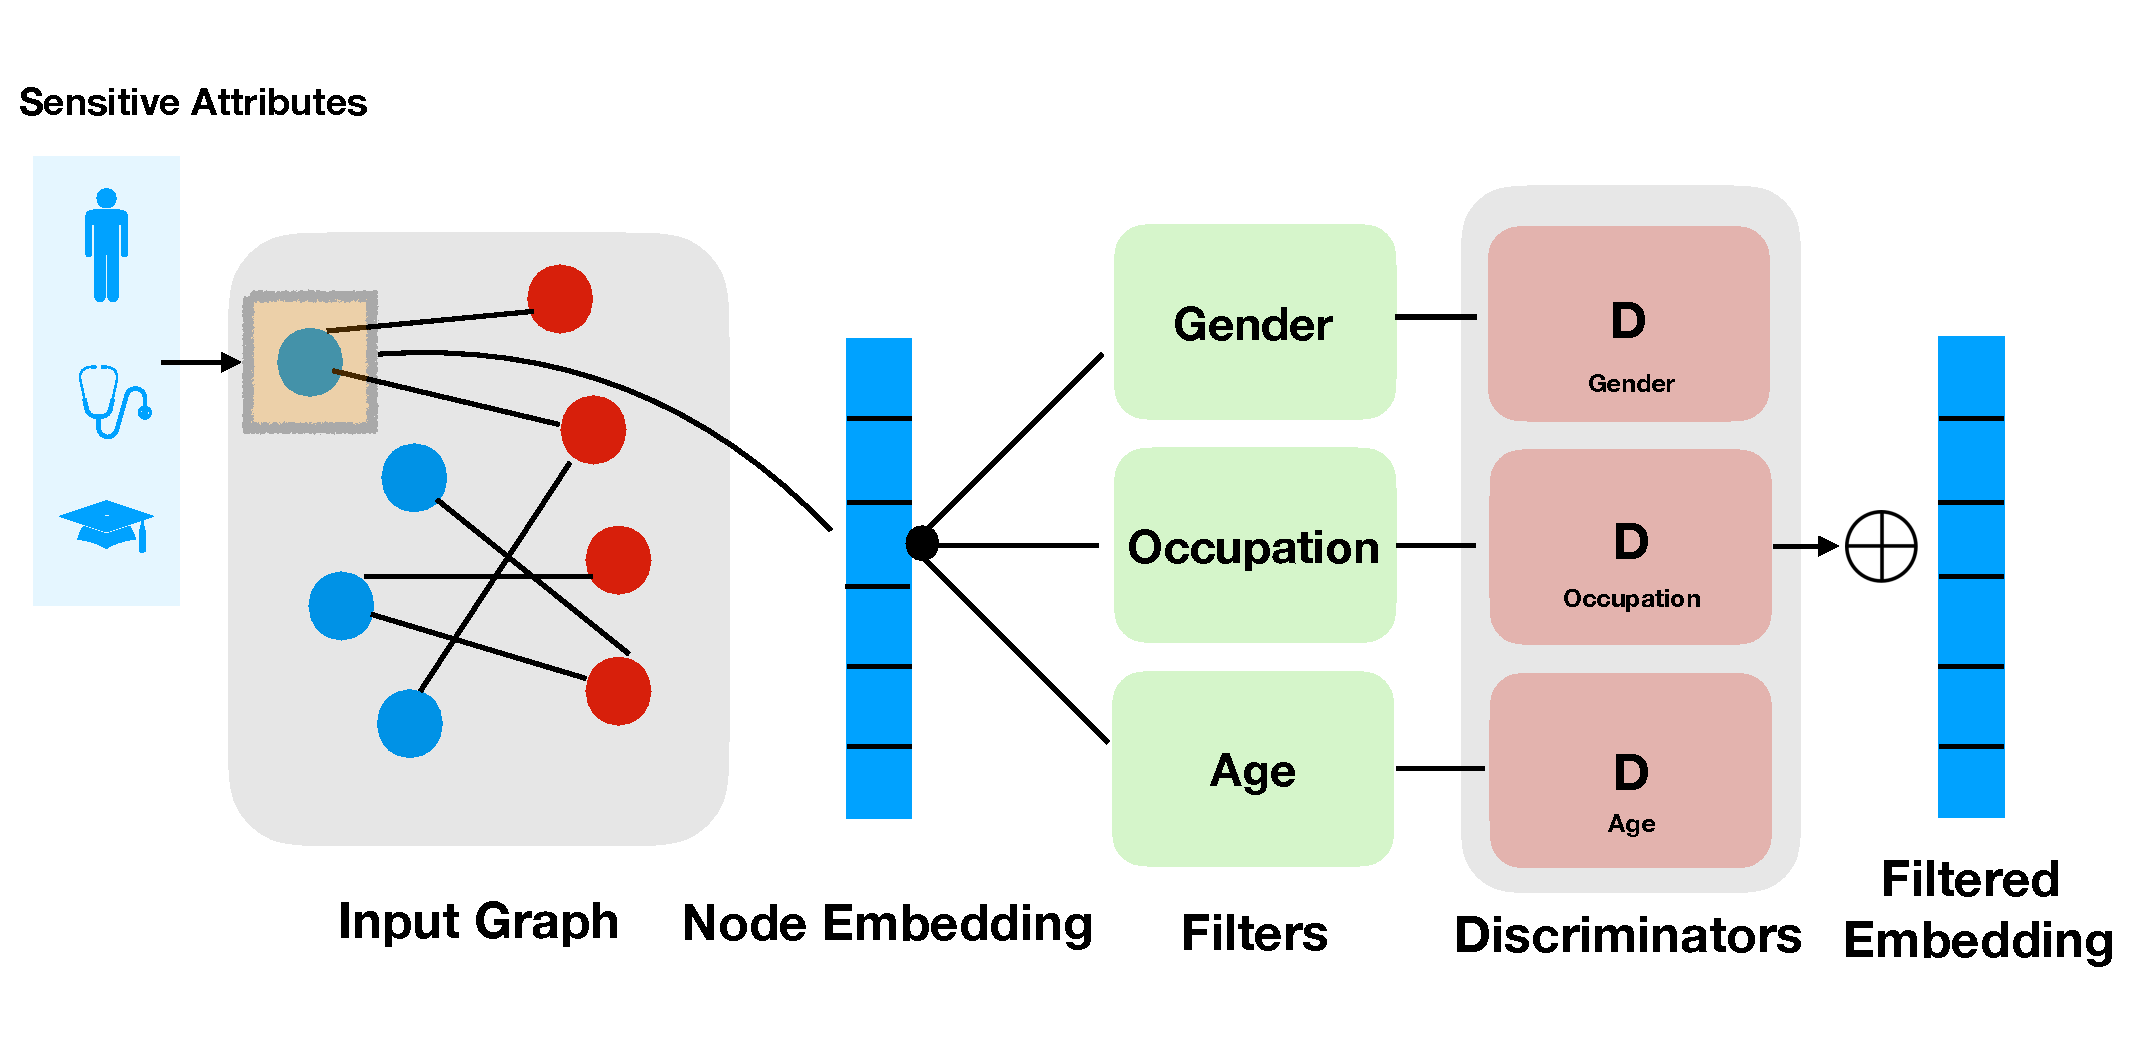
\includegraphics[width=1\linewidth]{icml2019_style/paper/plots/LightningTalk-Graphic.pdf}
    \vspace{-5mm}
    \caption{Compositional Adversary Architecture}
    \label{arch}
\end{figure}

\xhdr{Theoretical intuitions}
For clarity and simplicity, we consider the case of a single binary sensitive attribute, with the theoretical intuitions naturally generalizing to the multi-attribute and multi-class settings.
Assuming a single binary sensitive attribute $a_k$, by simple application of Proposition 2 in \citet{goodfellow2014generative}, we have:
\begin{theorem}
If $\compenc$ and $D_k$ have enough capacity, $T'$ is large enough so that $D_k$
is allowed to reach its optimum on $-L(e)$ (with $\compenc$ fixed), and $\compenc$ is optimized according to $L(e)$ (with $D$ fixed), then $I(\mb{z}_u, a_u) \rightarrow 0, \forall u \in \T^*$ as $\lambda \rightarrow \infty$. 
\end{theorem}
That is, if we increase the weight of the adversarial regularizer to infinity, the equilibrium of the minimax game in Equation \eqref{eq:loss} occurs when there is zero mutual information between the sensitive attribute and the embeddings. 
Of course, as $\lambda \rightarrow \infty$ trivial solutions to thie game exist (e.g., $\compenc$ simply outputting a constant value) and in practice setting $\lambda < \infty$ leads to a tradeoff between performance on edge prediction and representational invariance.
Theorem 1 holds as a consequence of Proposition 2 in \citet{goodfellow2014generative} if we simply replace the task of distinguishing real/fake data by classifying a binary sensitive attribute. 